\\[0.1in]
برای اینکه نشان بدهیم زبانی منظم است باید نشان دهیم که 
\lr{finite automation}
ای وجود دارد که زبان را تشخیص 
\LTRfootnote{recognize}
می‌دهد. همچنین به طور کلی برای $DFA$ها می‌دانیم:
\\
\begin{figure} [H]
    \centering
    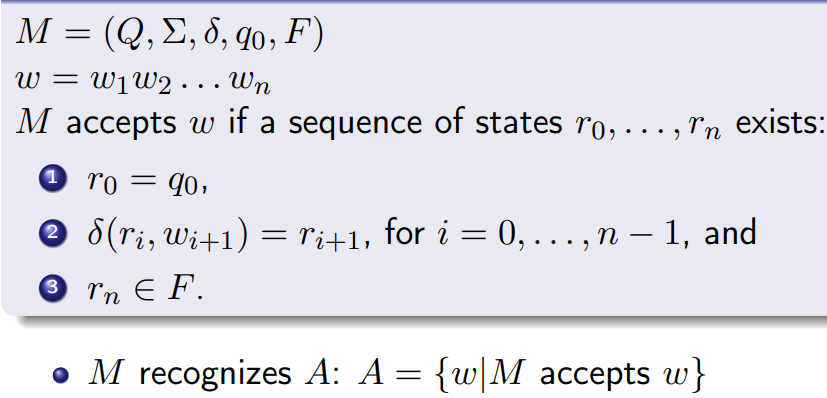
\includegraphics[scale=0.65]{solution/5-1.png}
    \caption{DFA}
    \label{dfa}
\end{figure}
\begin{enumerate}
    \item[1.]
    برای این زبان $NFA$ زیر را رسم می‌نماییم:\\[0.1in]
\begin{center}
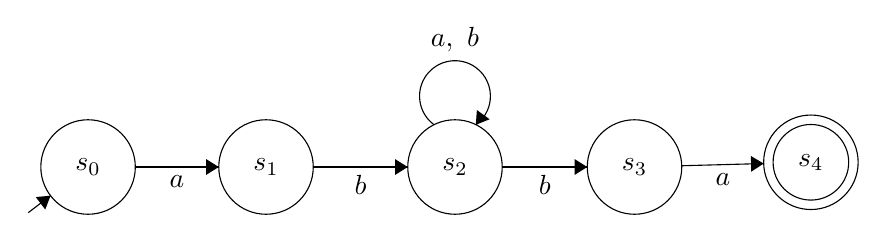
\begin{tikzpicture}[scale=0.2]
\tikzstyle{every node}+=[inner sep=0pt]
\draw [black] (13,-32.7) circle (3);
\draw (13,-32.7) node {$s_0$};
\draw [black] (24.3,-32.7) circle (3);
\draw (24.3,-32.7) node {$s_1$};
\draw [black] (36.3,-32.7) circle (3);
\draw (36.3,-32.7) node {$s_2$};
\draw [black] (47.7,-32.7) circle (3);
\draw (47.7,-32.7) node {$s_3$};
\draw [black] (58.9,-32.4) circle (3);
\draw (58.9,-32.4) node {$s_4$};
\draw [black] (58.9,-32.4) circle (2.4);
\draw [black] (9.2,-35.6) -- (10.62,-34.52);
\fill [black] (10.62,-34.52) -- (9.68,-34.61) -- (10.28,-35.4);
\draw [black] (16,-32.7) -- (21.3,-32.7);
\fill [black] (21.3,-32.7) -- (20.5,-32.2) -- (20.5,-33.2);
\draw (18.65,-33.2) node [below] {$a$};
\draw [black] (27.3,-32.7) -- (33.3,-32.7);
\fill [black] (33.3,-32.7) -- (32.5,-32.2) -- (32.5,-33.2);
\draw (30.3,-33.2) node [below] {$b$};
\draw [black] (34.977,-30.02) arc (234:-54:2.25);
\draw (36.3,-25.45) node [above] {$a,\mbox{ }b$};
\fill [black] (37.62,-30.02) -- (38.5,-29.67) -- (37.69,-29.08);
\draw [black] (39.3,-32.7) -- (44.7,-32.7);
\fill [black] (44.7,-32.7) -- (43.9,-32.2) -- (43.9,-33.2);
\draw (42,-33.2) node [below] {$b$};
\draw [black] (50.7,-32.62) -- (55.9,-32.48);
\fill [black] (55.9,-32.48) -- (55.09,-32) -- (55.11,-33);
\draw (53.31,-33.07) node [below] {$a$};
\end{tikzpicture}
\\[0.2in]
\end{center}
زبان $L$، زبانی است که رشته‌هایی را می‌پذیرد که حتما با $ab$ شروع بشوند و حتما با $ba$ خاتمه بیابند. به همین دلیل در $NFA$ رسم شده، ابتدا و به ترتیب با مشاهده کردن حروف 
$a$ و $b$ به استیت $s_2$ می‌رسیم.
بعد از آن از خواص $NFA$ کمک می‌گیریم. می‌توانیم با دیدن هر حروف از الفبای زبان، به خود $s_2$ برگردیم و یا اگر به طور متوالی $ba$ را دیدیم و رشته به پایان رسید، آن را $accept$ نماییم.
حال به تعریف کامل $NFA$ خود می‌پردازیم:\\[0.1in]
\begin{center}
    $N = (Q, \Sigma, \delta, q_0, F)$
    \begin{equation*}
    \begin{cases}
        Q &= \{ s_0, s_1, s_2, s_3, s_4\} \\
        \Sigma &= \{ a, b\} \\[0.15in]
        \delta &=
        \begin{tabular}{c|c|c}
         & $a$ & $b$ \\ \hline
        $s_0$ & $\{s_1\}$ &$\varnothing$\\
        $s_1$ & $\varnothing$ &$\{s_2\}$\\
        $s_2$ & $\{s_2\}$ &$\{s_2, s_3\}$\\
        $s_3$ & $\{s_4\}$ &$\varnothing$\\
        $s_4$ & $\varnothing$ &$\varnothing$ \\
        \end{tabular}\\[0.1in]
        q_0 &= s_0\\
        F &= \{s_4\}\\
    \end{cases}
    \end{equation*}
    \\[0.3in]
\end{center}
حال ثابت می‌نماییم که این ماشین زبان گفته شده را تشخیص می‌دهد.
برای یک $NFA$ می‌دانیم:\newline
\begin{figure} [H]
    \centering
    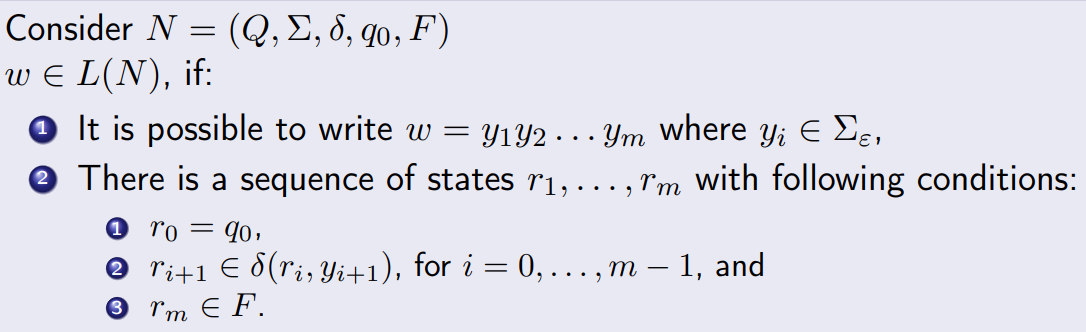
\includegraphics[scale=0.65]{solution/5-2.png}
        \caption{NFA}
    \label{nfa}
\end{figure}
حال به کمک استقرا، ماشین رسم شده و به روش زیر، اثبات را تکمیل می‌نماییم:\\[0.1in]
\begin{enumerate}
    \item[1.] پایه استقرا:\\[0.1in]
    اگر $w = \epsilon$، آنگاه رشته ایجاد شده $abba$ می‌باشد که ماشین $N$ آن را تشخیص می‌دهد. داریم:\\[0.1in]
    \begin{center}
        $s_0 \xrightarrow{a} s_1 \xrightarrow{b} s_2
        \xrightarrow{b} s_3 \xrightarrow{a} s_4$
    \end{center}
    در نتیجه تشخیص داده می‌شود.
    \\[0.05in]
    \item[2.] گام استقرا:\\[0.1in]
    فرض می‌کنیم که این ماشین، رشته ایجاد شده توسط زیررشته به طول $k$ را تشخیص می‌دهد.
    درواقع فرض می‌کنیم $w = r_1r_2\ldots r_k$. داریم:\\[0.1in]
    \begin{center}
        $l_1 = abr_1r_2\ldots r_kba$\\[0.07in]
        $\Longrightarrow s_0 \xrightarrow{a} s_1 \xrightarrow{b}
        s_2 \xrightarrow{r_1} s_2 \; \ldots \; \xrightarrow{r_k}
        s_2 \xrightarrow{b} s_3 \xrightarrow{a} s_4
        $\\[0.1in]
    \end{center}
\end{enumerate}
حال کافی است نشان دهیم که به ازای $w = r_1r_2\ldots r_kr_{k+1}$ نیز رشته ایجاد شده را تشخیص می‌دهیم. داریم:
\begin{center}
    $\delta(s_2, a) = {s_2},\;\;\;\delta(s_2, b) = {s_2, s_3}$\\[0.1in]
\end{center}
بنابراین با دریافت هر حرفی، می‌توانیم در $s_2$ بمانیم. بنابراین با دریافت $r_{k+1}$ داریم:\\[0.05in]
\begin{center}
    $l_2 = abr_1r_2\ldots r_kba$\\[0.07in]
    $\Longrightarrow s_0 \xrightarrow{a} s_1 \xrightarrow{b}
    s_2 \xrightarrow{r_1} s_2 \; \ldots \; \xrightarrow{r_k}
    s_2 \xrightarrow{r_{k+1}} s_2 \xrightarrow{b} s_3 \xrightarrow{a} s_4
    $\\[0.1in]
\end{center}
در نتیجه این رشته را نیز تشخیص می‌دهد و نشان دادیم که ماشین $N$ این این زبان را تشخیص می‌دهد و:\\[0.1in]
\begin{center}
    $L(N) = L \longrightarrow \text{\lr{L is regular}}.$\\[0.15in]
\end{center}
$\;*$نکته: می‌دانیم هر $NFA$ یک $DFA$ معادل دارد. همین‌که نشان دادیم زبان داده شده یک ماشین $NFA$ دارد برای منظم بودن آن کافی است اما برای \underline{کار اضافه‌تر} نشان می‌دهیم یک $DFA$ معادل نیز دارد و آن را از تبدیل $NFA$ رسم شده به $DFA$ به‌دست می‌آوریم. $DFA$ معادل به شکل زیر می‌باشد:
\\[0.1in]
\begin{center}
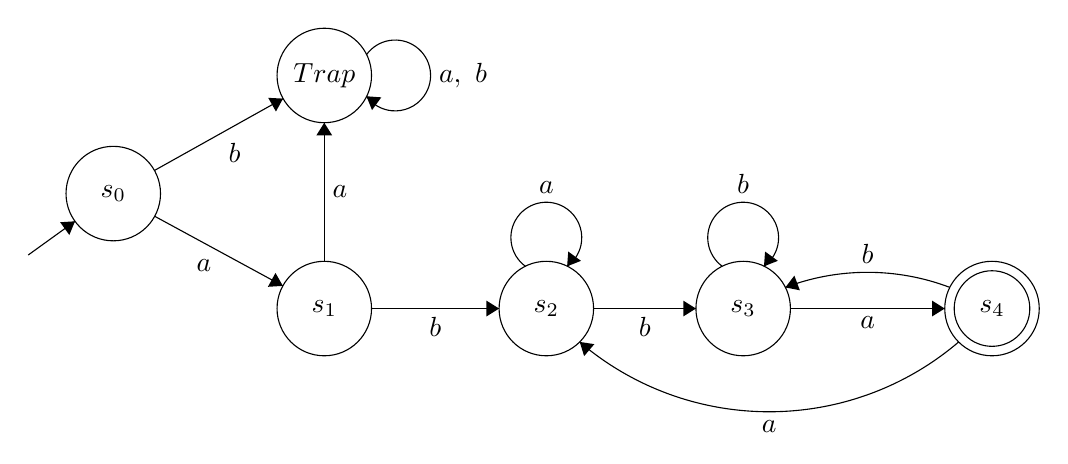
\begin{tikzpicture}[scale=0.2]
\tikzstyle{every node}+=[inner sep=0pt]
\draw [black] (13.5,-19.1) circle (3);
\draw (13.5,-19.1) node {$s_0$};
\draw [black] (26.9,-11.6) circle (3);
\draw (26.9,-11.6) node {$Trap$};
\draw [black] (26.9,-26.4) circle (3);
\draw (26.9,-26.4) node {$s_1$};
\draw [black] (41,-26.4) circle (3);
\draw (41,-26.4) node {$s_2$};
\draw [black] (53.5,-26.4) circle (3);
\draw (53.5,-26.4) node {$s_3$};
\draw [black] (69.3,-26.4) circle (3);
\draw (69.3,-26.4) node {$s_4$};
\draw [black] (69.3,-26.4) circle (2.4);
\draw [black] (8.1,-23) -- (11.07,-20.86);
\fill [black] (11.07,-20.86) -- (10.13,-20.92) -- (10.71,-21.73);
\draw [black] (16.12,-17.63) -- (24.28,-13.07);
\fill [black] (24.28,-13.07) -- (23.34,-13.02) -- (23.83,-13.89);
\draw (21.2,-15.85) node [below] {$b$};
\draw [black] (16.13,-20.54) -- (24.27,-24.96);
\fill [black] (24.27,-24.96) -- (23.8,-24.14) -- (23.32,-25.02);
\draw (19.26,-23.25) node [below] {$a$};
\draw [black] (26.9,-23.4) -- (26.9,-14.6);
\fill [black] (26.9,-14.6) -- (26.4,-15.4) -- (27.4,-15.4);
\draw (27.4,-19) node [right] {$a$};
\draw [black] (29.9,-26.4) -- (38,-26.4);
\fill [black] (38,-26.4) -- (37.2,-25.9) -- (37.2,-26.9);
\draw (33.95,-26.9) node [below] {$b$};
\draw [black] (29.58,-10.277) arc (144:-144:2.25);
\draw (34.15,-11.6) node [right] {$a,\mbox{ }b$};
\fill [black] (29.58,-12.92) -- (29.93,-13.8) -- (30.52,-12.99);
\draw [black] (39.677,-23.72) arc (234:-54:2.25);
\draw (41,-19.15) node [above] {$a$};
\fill [black] (42.32,-23.72) -- (43.2,-23.37) -- (42.39,-22.78);
\draw [black] (44,-26.4) -- (50.5,-26.4);
\fill [black] (50.5,-26.4) -- (49.7,-25.9) -- (49.7,-26.9);
\draw (47.25,-26.9) node [below] {$b$};
\draw [black] (52.177,-23.72) arc (234:-54:2.25);
\draw (53.5,-19.15) node [above] {$b$};
\fill [black] (54.82,-23.72) -- (55.7,-23.37) -- (54.89,-22.78);
\draw [black] (56.5,-26.4) -- (66.3,-26.4);
\fill [black] (66.3,-26.4) -- (65.5,-25.9) -- (65.5,-26.9);
\draw (61.4,-26.9) node [below] {$a$};
\draw [black] (67.184,-28.522) arc (-49.5514:-130.4486:18.549);
\fill [black] (43.12,-28.52) -- (43.4,-29.42) -- (44.05,-28.66);
\draw (55.15,-33.46) node [below] {$a$};
\draw [black] (56.177,-25.057) arc (110.79291:69.20709:14.713);
\fill [black] (56.18,-25.06) -- (57.1,-25.24) -- (56.75,-24.31);
\draw (61.4,-23.6) node [above] {$b$};
\end{tikzpicture}
\\[0.2in]
\end{center}
دقیقا همان مراحل استقرا را برای اثبات می‌توان برای این ماشین طی کرد.\\[0.1in]
\begin{enumerate}
    \item[1.] پایه استقرا:\\[0.1in]
    اگر $w = \epsilon$، آنگاه رشته ایجاد شده $abba$ می‌باشد که ماشین $DFA$ آن را تشخیص می‌دهد. داریم:\\[0.1in]
    \begin{center}
        $s_0 \xrightarrow{a} s_1 \xrightarrow{b} s_2
        \xrightarrow{b} s_3 \xrightarrow{a} s_4$
    \end{center}
    در نتیجه تشخیص داده می‌شود.
    \\[0.05in]
    \item[2.] گام استقرا:\\[0.1in]
    فرض می‌کنیم که این ماشین، رشته ایجاد شده توسط زیررشته به طول $k$ را تشخیص می‌دهد.
    درواقع فرض می‌کنیم $w = r_1r_2\ldots r_k$. تفاوت $DFA$ و $NFA$ در اینجا مشخص می‌شود که هنگامی که به استیت $s_2$ می‌رسیم، مانند $NFA$ با هر ورودی‌ای در همان استیت نمی‌مانیم. اگر $a$ دریاف کنیم در همان استیت می‌مانیم. به محض دیدن اولین $b$ به استیت $s_3$ خواهیم رفت. حال اگر $b$ ببینیم در همان استیت می‌مانیم اما اگر $a$ را ببینیم به استیت نهایی خواهیم رفت. حال اگر رشته تمام شده باشد که تشخیص داده‌ایم. در غیر این صورت اگر $a$ ببینیم به استیت $s_2$ و اگر $b$ ببینیم به استیت $s_3$ باز می‌گردیم و همان مراحل را طی می‌کنیم. بنابراین اگر رشته $l_1 = abr_1r_2\ldots r_kba$
    تشخیص داده شود، هنگام دیدن رشته $r_k$ یا به استیت $s_2$ می‌رویم یا در استیت $s_3$ خواهیم بود.
\end{enumerate}
حال اگر یک حرف $r_{k+1}$ اضافه بشود، طبق گفته‌های قبلی، ماشین رسم شده همچنان رشته را تشخیص می‌دهد. 
( به دلیل اینکه مراحل را به طور جزئی‌تر برای $NFA$ نشان دادیم، در این بخش از توضیح اضافه خودداری می‌نماییم.)\\[0.15in]
\item[2.]
برای این زبان $DFA$ زیر را رسم می‌نماییم:\\[0.1in]
\begin{center}
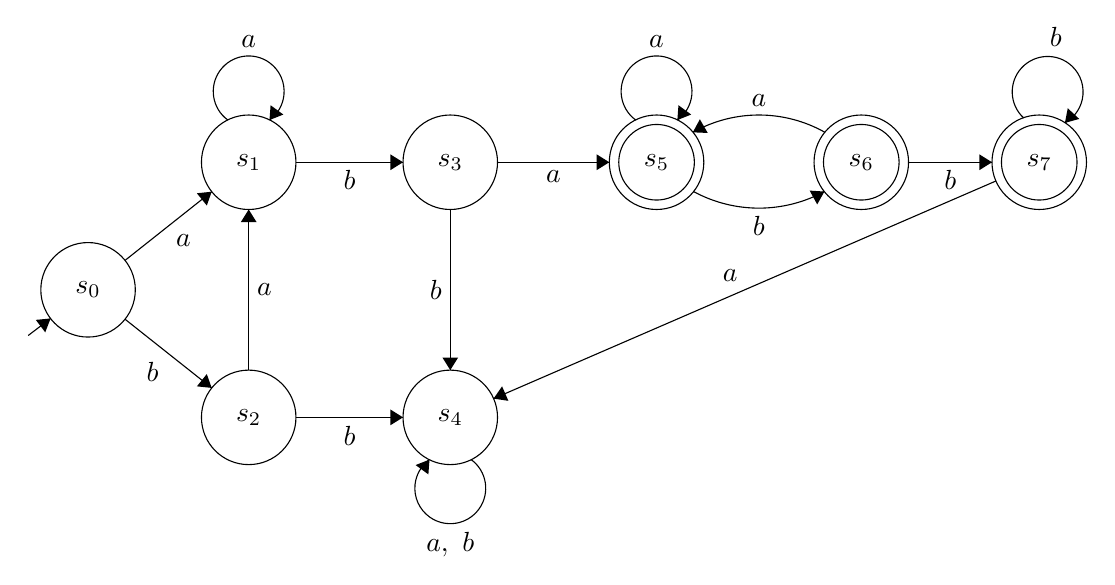
\begin{tikzpicture}[scale=0.2]
\tikzstyle{every node}+=[inner sep=0pt]
\draw [black] (11.5,-28.5) circle (3);
\draw (11.5,-28.5) node {$s_0$};
\draw [black] (21.7,-20.4) circle (3);
\draw (21.7,-20.4) node {$s_1$};
\draw [black] (21.7,-36.6) circle (3);
\draw (21.7,-36.6) node {$s_2$};
\draw [black] (34.5,-20.4) circle (3);
\draw (34.5,-20.4) node {$s_3$};
\draw [black] (47.6,-20.4) circle (3);
\draw (47.6,-20.4) node {$s_5$};
\draw [black] (47.6,-20.4) circle (2.4);
\draw [black] (34.5,-36.6) circle (3);
\draw (34.5,-36.6) node {$s_4$};
\draw [black] (60.6,-20.4) circle (3);
\draw (60.6,-20.4) node {$s_6$};
\draw [black] (60.6,-20.4) circle (2.4);
\draw [black] (71.9,-20.4) circle (3);
\draw (71.9,-20.4) node {$s_7$};
\draw [black] (71.9,-20.4) circle (2.4);
\draw [black] (7.7,-31.4) -- (9.12,-30.32);
\fill [black] (9.12,-30.32) -- (8.18,-30.41) -- (8.78,-31.2);
\draw [black] (13.85,-26.63) -- (19.35,-22.27);
\fill [black] (19.35,-22.27) -- (18.41,-22.37) -- (19.04,-23.15);
\draw (17.55,-24.95) node [below] {$a$};
\draw [black] (13.85,-30.37) -- (19.35,-34.73);
\fill [black] (19.35,-34.73) -- (19.04,-33.85) -- (18.41,-34.63);
\draw (15.59,-33.05) node [below] {$b$};
\draw [black] (24.7,-20.4) -- (31.5,-20.4);
\fill [black] (31.5,-20.4) -- (30.7,-19.9) -- (30.7,-20.9);
\draw (28.1,-20.9) node [below] {$b$};
\draw [black] (37.5,-20.4) -- (44.6,-20.4);
\fill [black] (44.6,-20.4) -- (43.8,-19.9) -- (43.8,-20.9);
\draw (41.05,-20.9) node [below] {$a$};
\draw [black] (21.7,-33.6) -- (21.7,-23.4);
\fill [black] (21.7,-23.4) -- (21.2,-24.2) -- (22.2,-24.2);
\draw (22.2,-28.5) node [right] {$a$};
\draw [black] (24.7,-36.6) -- (31.5,-36.6);
\fill [black] (31.5,-36.6) -- (30.7,-36.1) -- (30.7,-37.1);
\draw (28.1,-37.1) node [below] {$b$};
\draw [black] (35.823,-39.28) arc (54:-234:2.25);
\draw (34.5,-43.85) node [below] {$a,\mbox{ }b$};
\fill [black] (33.18,-39.28) -- (32.3,-39.63) -- (33.11,-40.22);
\draw [black] (34.5,-23.4) -- (34.5,-33.6);
\fill [black] (34.5,-33.6) -- (35,-32.8) -- (34,-32.8);
\draw (34,-28.5) node [left] {$b$};
\draw [black] (20.377,-17.72) arc (234:-54:2.25);
\draw (21.7,-13.15) node [above] {$a$};
\fill [black] (23.02,-17.72) -- (23.9,-17.37) -- (23.09,-16.78);
\draw [black] (46.277,-17.72) arc (234:-54:2.25);
\draw (47.6,-13.15) node [above] {$a$};
\fill [black] (48.92,-17.72) -- (49.8,-17.37) -- (48.99,-16.78);
\draw [black] (58.261,-22.255) arc (-61.44456:-118.55544:8.706);
\fill [black] (58.26,-22.26) -- (57.32,-22.2) -- (57.8,-23.08);
\draw (54.1,-23.81) node [below] {$b$};
\draw [black] (63.6,-20.4) -- (68.9,-20.4);
\fill [black] (68.9,-20.4) -- (68.1,-19.9) -- (68.1,-20.9);
\draw (66.25,-20.9) node [below] {$b$};
\draw [black] (70.905,-17.582) arc (227.18022:-60.81978:2.25);
\draw (72.96,-13.11) node [above] {$b$};
\fill [black] (73.53,-17.9) -- (74.44,-17.65) -- (73.71,-16.97);
\draw [black] (69.15,-21.59) -- (37.25,-35.41);
\fill [black] (37.25,-35.41) -- (38.19,-35.55) -- (37.79,-34.63);
\draw (52.28,-27.99) node [above] {$a$};
\draw [black] (49.903,-18.502) arc (119.43285:60.56715:8.541);
\fill [black] (49.9,-18.5) -- (50.85,-18.54) -- (50.35,-17.67);
\draw (54.1,-16.9) node [above] {$a$};
\end{tikzpicture}
\\[0.2in]
\end{center}
اگر بخواهیم توضیحی کلی برای $DFA$ رسم شده بدهیم، این‌گونه عمل می‌کند که
در هر حالتی، اگر رشته $aba$ را مشاهده نکرده باشد اما حداقل دو $b$ متوالی ببیند، 
به استیت $s_4$ خواهد رفت و هیچ‌گاه $accept$ نخواهد شد.
زیرا یا $bba$ را خواهد داشت و یا $aba$ را نخواهد دید. اما اگر به استیت 
$s_5$ برسیم، یعنی قطعا 
$aba$ را مشاهده کرده‌ایم. حال باید حالاتی که $bba$ را بعد از آن داریم حذف نماییم که اگر به استیت $s_7$ برسیم یعنی قطعا دو $b$ را دیده‌ایم. اگر دیگر $a$ نبینیم، باز در حالت درستی هستیم اما اگر $a$ را ببینیم، پاسخ باید $reject$ بشود زیرا $bba$ مشاهده شده است.
حال به تعریف کامل $DFA$ خود می‌پردازیم:\\[0.1in]
\begin{center}
    $M = (Q, \Sigma, \delta, q_0, F)$
    \begin{equation*}
    \begin{cases}
        Q &= \{ s_0, s_1, s_2, s_3, s_4, s_5, s_6, s_7\} \\
        \Sigma &= \{ a, b\} \\[0.15in]
        \delta &=
        \begin{tabular}{c|c|c}
         & $a$ & $b$ \\ \hline
        $s_0$ & $s_1$ &$s_2$\\
        $s_1$ & $s_1$ &$s_3$\\
        $s_2$ & $s_1$ &$s_4$\\
        $s_3$ & $s_5$ &$s_4$\\
        $s_4$ & $s_4$ &$s_4$\\
        $s_5$ & $s_5$ &$s_6$\\
        $s_6$ & $s_5$ &$s_7$\\
        $s_7$ & $s_4$ &$s_7$\\
        \end{tabular}\\[0.1in]
        q_0 &= s_0\\
        F &= \{s_5, s_6, s_7\}\\
    \end{cases}
    \end{equation*}
    \\[0.3in]
\end{center}
حال برای اثبات اینکه این ماشین زبان داده شده را تشخیص می‌دهد به کمک استقرا و شکل \ref{dfa} داریم:\\[0.05in]
\begin{enumerate}
    \item[1.] پایه استقرا:\\[0.1in]
    اگر $w = aba$، آنگاه رشته ایجاد شده $aba$ می‌باشد که ماشین $M$ آن را تشخیص می‌دهد. داریم:\\[0.1in]
    \begin{center}
        $s_0 \xrightarrow{a} s_1 \xrightarrow{b} s_3
        \xrightarrow{a} s_5$
    \end{center}
    در نتیجه تشخیص داده می‌شود.
    \\[0.05in]
    \item[2.] گام استقرا:\\[0.1in]
    فرض می‌کنیم که این ماشین، رشته ایجاد شده توسط زیررشته به طول $k$ را تشخیص می‌دهد.
    درواقع فرض می‌کنیم $w = r_1r_2aba\ldots r_{k-2}$. داریم:\\[0.1in]
    \begin{center}
        $w = r_1r_2aba\ldots r_{k-3}$\\[0.07in]
        $r_{k-3}\;\in\;\{s_5,s_6,s_7\}$\\[0.15in]
    \end{center}
\end{enumerate}
حال باید برای $w = r_1r_2aba\ldots r_{k-3}r_{k-2}$ اثبات نماییم که $M$ آن را تشخیص خواهد داد.
همانطور که اشاره کردیم $r_{k-3}$ در یکی از استیت‌های $s_5$ یا $s_6$ یا $s_7$
حضور دارد. همچنین می‌دانیم $r_i\;\in\;\{a,b\}$. بنابراین 3 حالت پیش خواهد آمد:
\newline
\begin{itemize}
    \item $r_{k-3}\in s_5$:
    در این حالت با ورودی گرفتن $a$ یا $b$ یا در $s_5$ خواهیم ماند و یا به $s_6$ خواهیم رفت که در هر دو حالت در استیت نهایی هستیم پس رشته تشخیص داده می‌شود.
    دلیل منطقی آن هم این است که ما تنها هنگامی در استیت $s_5$ هستیم که آخرین کاراکتر حتما $a$ بوده باشد. بنابراین چه با دریافت $a$ و چه با دریافت $b$، زیررشته $bba$ به وجود نخواهد آمد و همچنان رشته تشخیص داده می‌شود.
    \item $r_{k-3}\in s_6$:
    در این حالت با ورودی گرفتن $a$ یا $b$ یا به $s_5$ خواهیم رفت و یا به $s_7$ خواهیم رفت که در هر دو حالت در استیت نهایی هستیم پس رشته تشخیص داده می‌شود.
    دلیل منطقی آن هم این است که ما هنگامی در $s_6$ هستیم که دو کاراکتر آخر $ab$ باشند:
    \\[0.05in]
    \begin{center}
        $r_{k-4} = a,\;\;\;r_{k-3} = b$\\[0.1in]
    \end{center}
    حال با دریافت هر کدام از $a$ و یا $b$ زیررشته $bba$ تولید نمی‌شود؛ پس رشته مورد نظر همچنان تشخیص داده می‌شود.
    \item $r_{k-3}\in s_7$:
    ما هنگامی در این استیت خواهیم بود که دو کاراکتر اخر حتما $b$ باشند:
    \\[0.05in]
    \begin{center}
        $r_{k-4} = b,\;\;\;r_{k-3} = b$\\[0.1in]
    \end{center}
    در این حالت طبیعتا با دیدن $b$ مشکلی پیش نخواهد آمد و در همان استیت $s_7$ خواهیم ماند و رشته‌ای که قبلا تشخیص داده شده بود، اکنون نیز تشخیص داده می‌شود. اما اگر $a$ ببینیم، قطعا زیررشته $bba$  به وجود آمده است و ما به استیت $s_4$ که نهایی نیست می‌رویم و مطابق انتظار رشته تشخیص داده نمی‌شود.
\end{itemize}
بنابراین تمامی شروط مورد نیاز را نشان دادیم که اجرا می‌شود و با استقرا ثابت کردیم که این ماشین رشته‌های این زبان را تشخیص می‌دهد و زبان منظم است. توجه بفرمایید در هر دو بخش این پرسش و در بخش بعد، $s_0$ استیت شروع است. ترنزیشن‌ها یا همان $\delta$ برای هر ماشین نشان داده شده است و همچنین استیت‌های نهایی را نیز مشخص نموده‌ایم. پس شروط نشان‌داده شده در شکل‌های
\ref{dfa}و\ref{nfa} ارضا شده‌اند.
\\[0.1in]
\item[3.]
برای این زبان، $DFA$ زیر را رسم می‌کنیم:\\[0.1in]
\begin{center}
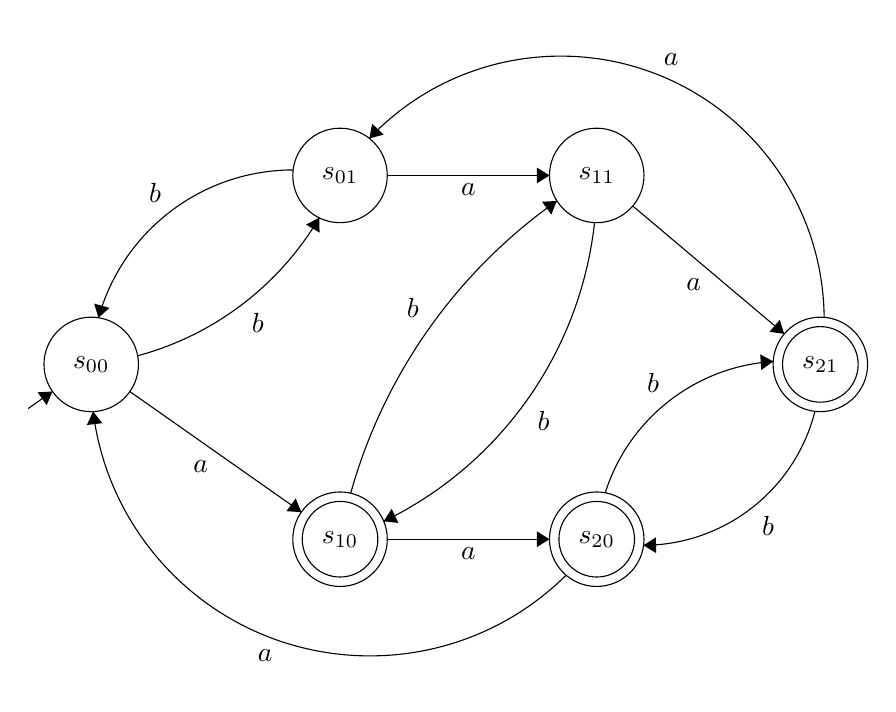
\begin{tikzpicture}[scale=0.2]
\tikzstyle{every node}+=[inner sep=0pt]
\draw [black] (13.5,-26.3) circle (3);
\draw (13.5,-26.3) node {$s_{00}$};
\draw [black] (29.3,-14.3) circle (3);
\draw (29.3,-14.3) node {$s_{01}$};
\draw [black] (29.3,-37.4) circle (3);
\draw (29.3,-37.4) node {$s_{10}$};
\draw [black] (29.3,-37.4) circle (2.4);
\draw [black] (45.6,-14.3) circle (3);
\draw (45.6,-14.3) node {$s_{11}$};
\draw [black] (59.8,-26.3) circle (3);
\draw (59.8,-26.3) node {$s_{21}$};
\draw [black] (59.8,-26.3) circle (2.4);
\draw [black] (45.6,-37.4) circle (3);
\draw (45.6,-37.4) node {$s_{20}$};
\draw [black] (45.6,-37.4) circle (2.4);
\draw [black] (27.98,-16.991) arc (-30.6027:-74.96442:19.182);
\fill [black] (27.98,-16.99) -- (27.14,-17.42) -- (28,-17.93);
\draw (24.08,-23) node [below] {$b$};
\draw [black] (15.95,-28.02) -- (26.85,-35.68);
\fill [black] (26.85,-35.68) -- (26.48,-34.81) -- (25.9,-35.62);
\draw (20.45,-32.35) node [below] {$a$};
\draw [black] (13.961,-23.343) arc (164.43873:89.99415:12.835);
\fill [black] (13.96,-23.34) -- (14.66,-22.71) -- (13.69,-22.44);
\draw (17.56,-16.07) node [above] {$b$};
\draw [black] (32.3,-14.3) -- (42.6,-14.3);
\fill [black] (42.6,-14.3) -- (41.8,-13.8) -- (41.8,-14.8);
\draw (37.45,-14.8) node [below] {$a$};
\draw [black] (29.977,-34.478) arc (164.40768:125.17661:33.834);
\fill [black] (43.07,-15.92) -- (42.13,-15.97) -- (42.71,-16.79);
\draw (34.33,-22.7) node [left] {$b$};
\draw [black] (47.89,-16.24) -- (57.51,-24.36);
\fill [black] (57.51,-24.36) -- (57.22,-23.47) -- (56.57,-24.23);
\draw (51.75,-20.79) node [below] {$a$};
\draw [black] (45.46,-17.295) arc (-6.26003:-64.15568:23.983);
\fill [black] (32.07,-36.26) -- (33.01,-36.37) -- (32.58,-35.47);
\draw (41.81,-29.87) node [right] {$b$};
\draw [black] (32.3,-37.4) -- (42.6,-37.4);
\fill [black] (42.6,-37.4) -- (41.8,-36.9) -- (41.8,-37.9);
\draw (37.45,-37.9) node [below] {$a$};
\draw [black] (43.657,-39.681) arc (-45.26879:-172.88141:17.711);
\fill [black] (13.62,-29.29) -- (13.22,-30.15) -- (14.21,-30.03);
\draw (24.55,-44.37) node [below] {$a$};
\draw [black] (46.139,-34.457) arc (162.44458:93.5842:11.982);
\fill [black] (56.81,-26.11) -- (55.98,-25.66) -- (56.05,-26.66);
\draw (49.18,-28.14) node [above] {$b$};
\draw [black] (31.157,-11.949) arc (136.55156:0.49486:16.736);
\fill [black] (31.16,-11.95) -- (32.07,-11.71) -- (31.34,-11.02);
\draw (50.33,-7.37) node [above] {$a$};
\draw [black] (59.459,-29.272) arc (-14.16866:-89.80256:11.275);
\fill [black] (48.57,-37.79) -- (49.37,-38.28) -- (49.36,-37.28);
\draw (56.48,-35.89) node [below] {$b$};
\draw [black] (9.5,-29.1) -- (11.04,-28.02);
\fill [black] (11.04,-28.02) -- (10.1,-28.07) -- (10.67,-28.89);
\end{tikzpicture}
\\[0.2in]
\end{center}
این ماشین باید رشته‌هایی را تشخیص بدهد که باقی‌مانده تعداد دفعات دیده شدن $a$ بر 3 از باقی‌مانده تعداد دفعات دیده شدن $b$ بر 2، بیشتر باشد. می‌دانیم باقی‌مانده بر 3، 3 حالت دارد و باقی‌مانده بر 2 نیز 2 حالت دارد. در شماره گذاری استیت‌های این $DFA$ از 
$s_{mn}$ استفاده نمودیم که به این معناست که در آن استیت،
باقی‌مانده تعداد $a$ بر 3 برابر با
$\;m$و باقی‌مانده تعداد $b$ بر 2 برابر با 
$n$ می‌باشد.\\
بنابراین در این حالت استیت‌هایی که در آن‌ها $m > n$ می‌باشد، استیت‌های نهایی هستند.\\
در هر استیت هم با دیدن $a$ به استیت
$s_{((m+1)\%3)n}$ می‌رویم و
اگر $b$ ببینیم به استیت
$s_{m((n+1)\%2)}$
خواهیم رفت.
حال به تعریف کامل $DFA$ خود می‌پردازیم:\\[0.1in]
\begin{center}
    $M = (Q, \Sigma, \delta, q_0, F)$
    \begin{equation*}
    \begin{cases}
        Q &= \{ s_{00}, s_{01}, s_{10}, s_{11}, s_{20}, s_{21}\} \\
        \Sigma &= \{ a, b\} \\[0.15in]
        \delta &=
        \begin{tabular}{c|c|c}
         & $a$ & $b$ \\ \hline
        $s_{00}$ & $s_{10}$ &$s_{01}$\\
        $s_{01}$ & $s_{11}$ &$s_{00}$\\
        $s_{10}$ & $s_{20}$ &$s_{11}$\\
        $s_{11}$ & $s_{21}$ &$s_{10}$\\
        $s_{20}$ & $s_{00}$ &$s_{21}$\\
        $s_{21}$ & $s_{01}$ &$s_{20}$\\
        \end{tabular}\\[0.1in]
        q_0 &= s_{00}\\
        F &= \{s_{10}, s_{20}, s_{21}\}\\
    \end{cases}
    \end{equation*}
    \\[0.2in]
\end{center}
حال برای اثبات اینکه این ماشین زبان داده شده را تشخیص می‌دهد به کمک استقرا و شکل \ref{dfa} داریم:\newline
( برای راحتی در نظر بگیرید: $n_a(w)\%3 = c, \;\; n_b(w)\%2=d$ )
\begin{enumerate}
    \item[1.] پایه استقرا:\\[0.1in]
    اگر $w = a$، آنگاه رشته ایجاد شده $a$ می‌باشد که ماشین $M$ آن را تشخیص می‌دهد. داریم:\\[0.05in]
    \begin{center}
        $s_{00} \xrightarrow{a} s_{10}$\\[0.05in]
    \end{center}
    در نتیجه تشخیص داده می‌شود. برای $aba$ نیز می‌توانیم نشان دهیم:\\[0.05in]
    \begin{center}
        $s_{00} \xrightarrow{a} s_{10} \xrightarrow{b} s_{11}
        \xrightarrow{a} s_{21}$\\[0.05in]
    \end{center}
    \item[2.] گام استقرا:\\[0.1in]
    فرض می‌کنیم که این ماشین، رشته ایجاد شده توسط زیررشته به طول $k$ را تشخیص می‌دهد.
    درواقع فرض می‌کنیم $w = r_1r_2\ldots r_{k}$. داریم:\\[0.1in]
    \begin{center}
        $w = r_1r_2\ldots r_{k}$\\[0.07in]
        $r_{k}\;\in\;\{s_{10},s_{20},s_{21}\}$\\[0.15in]
    \end{center}
\end{enumerate}
بنابراین برای $w = r_1r_2\ldots r_{k}r_{k+1}$ 3 حالت وجود دارد:\newline
\begin{itemize}
    \item $r_{k}\in s_{10}$:
    ما هنگامی در این استیت قرار داریم و کارمان به پایان می‌رسد که:\\[0.05in]
    \begin{center}
        $c = 1,\;\;\; d = 0$\newline
    \end{center}
    حال اگر $r_{k+1} = a$، آنگاه همچنان شرط خواسته شده سوال پابرجاست و به استیت
    $s_{20}$ می‌رویم که آن هم یک استیت تهایی می‌باشد. اما اگر 
    $r_{k+1} = b$، در آن صورت $c = b$ پس نباید رشته تشخیص داده بشود که ما نیز در این حالت به استیت $s_{11}$ می‌رویم که نهایی نیست.\newline
    \item $r_{k}\in s_{20}$:
        ما هنگامی در این استیت قرار داریم و کارمان به پایان می‌رسد که:\\[0.05in]
    \begin{center}
        $c = 2,\;\;\; d = 0$\newline
    \end{center}
    حال اگر $r_{k+1} = a$، آنگاه $c = 0$ و رشته نباید تشخیص داده بشود که ماشین نیز به درستی به استیت $s_{00}$ که نهایی نیست می‌رود.
    اما اگر $r_{k+1}=b$، آنگاه $d=1$ و همچنان $c>d$، بنابراین رشته باید تشخیص داده بشود که ماشین نیز به استیت $s_{21}$ که نهایی است می‌رود.\newline
    \item $r_{k}\in s_{21}$:
        ما هنگامی در این استیت قرار داریم و کارمان به پایان می‌رسد که:\\[0.05in]
    \begin{center}
        $c = 2,\;\;\; d = 1$\newline
    \end{center}
    حال اگر $r_{k+1} = a$، آنگاه $c = 0$ و رشته نباید تشخیص داده بشود که ماشین نیز به درستی به استیت $s_{01}$ که نهایی نیست می‌رود.
اما اگر $r_{k+1}=b$، آنگاه $d=0$ و همچنان $c>d$، بنابراین رشته باید تشخیص داده بشود که ماشین نیز به استیت $s_{20}$ که نهایی است می‌رود.\newline
\end{itemize}
بنابراین نشان دادیم که ماشین رسم شده زبان خواسته شده را تشخیص می‌دهد و زبان، منظم می‌باشد.
باز هم تاکید می‌نماییم که تمامی شروط ذکر شده در شکل \ref{dfa} برآورده شده است و در این بخش نیز استیت $s_{00}$ استیت آغازین می‌باشد.
\end{enumerate}